\section{Эксперименты}

С чего же начать???

% ----
Имплементация моделей, код для тренировки и валидации, функций потерь и метрик качества были написаны на языке Python 3.8
с использованием фреймворка для глубокого обучения Pytorch\cite{Pytorch}.

% про ббс 
В работе была использована оригинальная имплементации модели от авторов статьи \cite{BBS}, которая доступна на GitHub [ссылка!].
На её основе была написана модель BBS-Net, которая в качестве бэкбона использовала свёрточную нейронную сеть EfficientNet-B0 \cite{Efficientnet}.

% детали реализации надо? или описать это, когда модели описываем? 


Все модели тренировались и валидировались на датасете NJU2K предварительно разделённым на NJU2K\_TRAIN для тренировки, 
который содержит 1485 изображений, и NJU2K\_TRAIN для промежуточной валидации, содержащий 500 изображений.
Каждая тренировка состояла из 150 эпох с размером пакета(batch size) равным 10. В конце каждой эпохи запускалась валидация: рассчитывалось среднее
значение функции потерь и средней абсолютной ошибки(MAE), минимальное значение которой сохраняется и обновляется во время
всего процесса тренировки. В случае обновления значения - текущее состояние модели сохраняется и помечается наилучшим в смысле качества обучения.
В результате тренировки мы получаем модель, которая показывает наименьшую ошибку на валидационном датасете. Такая стратегия используется для того,
чтобы избежать переобучения под тренировочный датасет. 
Для тренировки модели использовался стандартный оптимизатор Adam\cite{Adam}. Начальное значение параметра скорости обучения(learning rate) 
равно 0.0001. Каждые 60 эпох значение уменьшалось в 10 раз \ref{fig:lr}. Такой подход был предложен в оригинальной работе \cite{BBS}.

\begin{figure}[h]
    \centering
    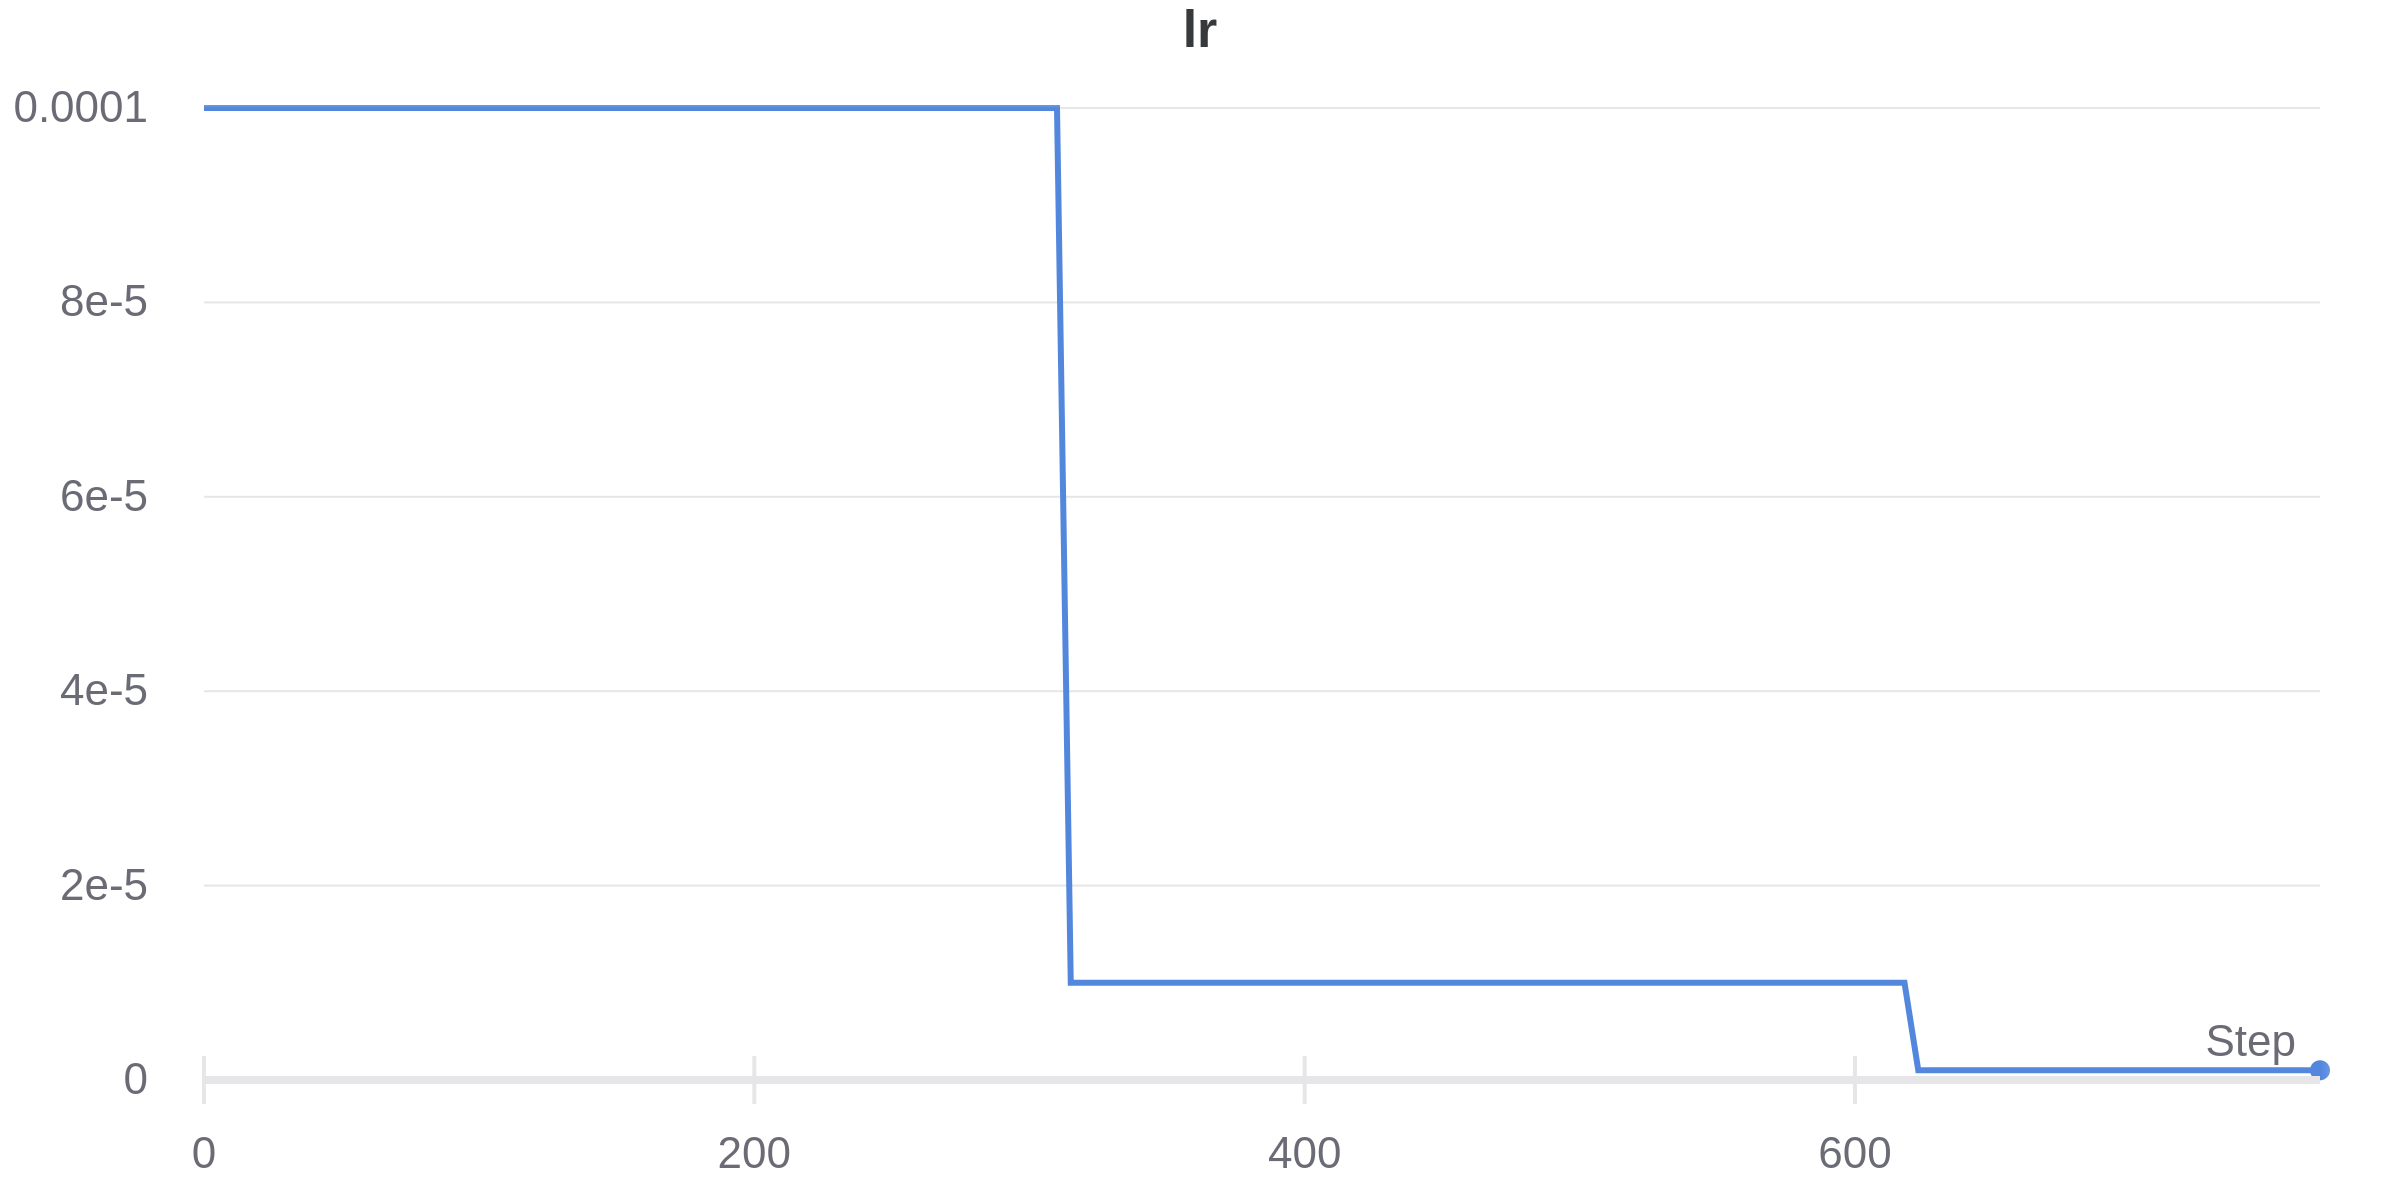
\includegraphics[width=1\textwidth]{lr}
    \caption{Изменения скорости обучения при тренировке}
    \label{fig:lr}
\end{figure}

На вход модели подаются RGB изображение и карта глубины с разрешением 352х352 как на этапе тренировки, там и на этапе расчёта тестовых метрик.
Так как изображения в датасетах имеют разные размеры, перед передачей применяется изменение размера, а также, на этапе тренировки, некоторые приёмы аугментации 
изображения: поворот, масштабирование, кроп. Все преобразования выполняются через стандартные классы для работы с данными в Pytorch: Dataset и DataLoader
\footnote{\url{https://pytorch.org/docs/stable/data.html}}
Все эксперименты проводились на платформе Google Colab\footnote{\url{https://colab.research.google.com/notebooks/intro.ipynb}}
с GPU Tesla P100-PCIE-16GB.



%Таблчика с экспериментами

\begin{center}
    \begin{table}
        \begin{tabular}{ |c c|c|c|c|c|c|c|c|c| } 
            \hline
            \multirow{2}{*}{\rotatebox[origin=c]{90}{Датасет}} & \multirow{2}{*}{Метрика} & \multicolumn{4}{ |c| }{ResNet} & \multicolumn{4}{ |c| }{EfficientNet} \\
            \cline{3-10}
            & & BCE & focal & dice & IoU & BCE & focal & dice & IoU\\
            \hline
            \multirow{2}{*}{\rotatebox[origin=c]{90}{NJU2K}} & mae $\downarrow$ &0,033&0,06&0,031&0,032&0,035&0.057&0,031&\textbf{0,030} \\
            & f1  $\uparrow$ &0,909&0,832&\textbf{0,920}&0,915&0,901&0.842&0,916&0,918\\
            \multirow{2}{*}{\rotatebox[origin=c]{90}{NLPR}} & mae $\downarrow$ &  & &  & &  & &  & \\
            & f1  $\uparrow$ & \textbf{0,920} & & & & & & &\\
            \multirow{2}{*}{\rotatebox[origin=c]{90}{DES}} & mae $\downarrow$ &0,019&0,041&0,017&\textbf{0,015}&0,019&0.039&0,016&0,016\\
            & f1  $\uparrow$ &0,916&0,819&0,930&\textbf{0,939}&0,918&0.822&0,933&0,929\\
            \multirow{2}{*}{\rotatebox[origin=c]{90}{SSD}} & mae $\downarrow$ &0,046&0,073&0,044&0,046&0,047&0.068&0,043&\textbf{0,041} \\
            & f1  $\uparrow$ &0,841&0.777&0,855&0,851&0,844&0.777&0,860&\textbf{0,863}\\
            \multirow{2}{*}{\rotatebox[origin=c]{90}{STERE}} & mae $\downarrow$ &0,039&0,066&0,037&\textbf{0,035}&0,039&0.063&0,037&0,036 \\
            & f1  $\uparrow$ &0,888&0,817&0,898&\textbf{0,905}&0,891&0.824&0,899&0,903\\   
            \multirow{2}{*}{\rotatebox[origin=c]{90}{LFSD}} & mae $\downarrow$ &0,077&0,104&\textbf{0,066}&0,072&0,074&0.102&0,082&0,072\\
            & f1  $\uparrow$ &0,843&0,782&\textbf{0,862}&0,859&0,843&0.789&0,834&0,851\\  
            \multirow{2}{*}{\rotatebox[origin=c]{90}{SIP}} & mae $\downarrow$ &0,047&0,07&0,045&0,044&0,047&0.069&0,051&\textbf{0,042}\\
            & f1  $\uparrow$ &0,867&0,789&0,877&0,88&0,87&0.809&0,859&\textbf{0,884}\\  
            \multirow{2}{*}{\rotatebox[origin=c]{90}{DUT}} & mae $\downarrow$ &0,121&0,145&0,116&0,121&0,112&0.122&\textbf{0,105}&0,14\\
            & f1  $\uparrow$ &0,592&0,574&0,67&0,597&0,65&0.639&0,707&\textbf{0,728}\\  
            \hline
        \end{tabular}
    \caption{Эксперименты}
    \label{tab:experiments}
    \end{table}
\end{center}



